\documentclass{article}
\usepackage[margin=2cm, includefoot, footskip=30pt]{geometry}
\setlength\parindent{0pt}
\setlength{\parskip}{1em}
\usepackage{authblk}
\usepackage{pdfpages}

\title{Stability of defection, optimisation of strategies and the limits of
memory in the Prisoner's Dilemma RESPONSE TO REVIEWS}

\author{Nikoleta E. Glynatsi, Vincent A. Knight}

\begin{document}

\maketitle

We would like to open this response by thanking the reviewers for their
thoughtful comments and suggestions. We have fully taken their comments on board
and made significant modifications to both the mathematical arguments and the narrative. We feel this has greatly improved the work.

Both reviewers commented on different aspects of the paper and so our modifications
naturally fit in to two categories (which we will discuss in detail comment by comment):

\begin{itemize}
    \item The first is an improvement of the theoretic results both in terms of
    their proofs but also the result themselves. For example, we omitted to
    include the derivative of a quadratic form in one of our proofs
    and also had only given that quadratic form for the specific case of \((R,
    P, T, S)=(3, 0, 5, 1)\). The reviewer was very right to point out issues
    like this and we feel that we have addressed them all.
    \item The second reviewer questioned the general narrative of the paper as
    well as the evolutionary work. This was very helpful and we took time to
    reflect on the narrative of the paper. As a result of this we have changed
    the title to ``A theory of mind: Best responses to memory-one strategies.
    The limitations of extortion and restricted memory'' and reorganised some of
    the content. We have also clarified the nature of the evolutionary process
    we're discussing.
\end{itemize}

We will now take each comment of the reviewers in turn and highlight our efforts
to improve the work.

\section{Response}

\textbf{Regarding the comments of Reviewer 1:}

\begin{verbatim}
     ``Theorem 2: First, it is not clear how equation 17 is obtained.''
\end{verbatim}

This comment points out that we had skipped a step in obtaining the dot product
of the state vector \(v\) and the payoff matrix \((R, S, T, P)\).
This has been added in the proof of what used to be Theorem 2 but is now Theorem 1.

\begin{verbatim}
    ``Theorem 2: Moreover, even if that's correct, it is only for a
    specific PD payoff matrix. One cannot state the general results in (4) from
    just a specific case. To obtain (4), authors need to establish it for the
    general PD payoff matrix.''
\end{verbatim}

We agree with the comment of the reviewer. The utility was
specific only for a given payoff matrix. We have generalised our result by
considering the generalised payoffs \((R, S, T, P)\) and agree that this a more useful
result and whilst we were worried that this closed form could be messy it is in fact relatively elegant.

\begin{verbatim}
     ``Theorem 3: The proof in the Appendix did not show how to obtain equations
    (22) - (24), the key results of the Theorem''
\end{verbatim}

Equations (22) - (24) relay on the derivative of the utility \(\sum\limits_{i=1}
^ N  u_q^{(i)}(p)\) which is a sum of quadratic form ratios. The derivative is
obtained by using the property \(\frac{d x A x^T}{dx} =  2Ax\). We have added
these details and a reference text in the proof.
\begin{verbatim}
     ``Theorem 3: and what was stated in (5)''
\end{verbatim}

We have added a sentence clarifying that this is obtained by taking the average
over the opponents of the previously obtained expression for the utility.

\textbf{Regarding the comments of Reviewer 2:}

\begin{verbatim}
    ``what exactly is the evolutionary process used, what are the parameters?
    This is not mentioned anywhere in the paper or appendix, and makes it then
    hard to evaluate the impact of the findings, or give any hope for reproducing
    the results. I realize that there is a repository containing raw data, but
    the lack of explanation of the setup really harms any expectation of the
    paper being self-contained. The issue of the evolutionary process not being
    explained also prevented me from fully following the argument the authors
    make for why best responses in the evolutionary process would be less
    extortionate. ''
\end{verbatim}

We agree with the comment of the reviewer. We are not running a evolutionary
process. We study best
responses to memory-one strategies that include self interactions which in a sense are
approximating evolutionary stable best response strategies. We have reworded
this part of the work to clarify that we are only considering the possibility of
including self interactions and our results in an evolutionary process. We also explain how this could be
used in a Moran process setting.

\begin{verbatim}
    ``Another related problem is that the authors don't go into more detail about
    their SSE method. A more expansive explanation (also of Table 1) would be of
    critical importance, seeing that this is one of the central points of the
    results section.''
\end{verbatim}

We have included details of the SSE method and a better
discussion of the results based on Table 1. We have also included plots of the
SSE distributions that accompany Table 1.

\begin{verbatim}
    ``Another point I want to raise is how this work relates to the findings in Hilbe
    et al.: Partners and rivals in direct reciprocity (Nature Human Behaviour,
    2018). That previous review article shows, among other results, the conditions
    under which "partner" (aiming for mutual cooperation, fighting back against
    defection) or "rival" (defecting/extortionate) strategies evolve in the IPD. It
    seems that the authors of the current work investigate a similar distinction
    (however, they should explain what exactly they mean with "adaptable", as it
    features as a contrast to "extortionate"), and thus would profit from discussing
    the Hilbe et al. article as well.
    ''
\end{verbatim}

We thank the reviewer for their article recommendation. The findings of Hilbe et
 al and how our results relate to them, are discussed in the ``Results'' section. % TODO Vince to add details

\begin{verbatim}
    ``As a last point, I think that the flow of the paper could be improved. As it is
    now, the paper reads a bit like a list of results that are more or less loosely
    tied together (especially Section 1.2 suffers from this problem in comparison to
    the others). It would be good to motivate single sections in the broader context
    of the message the paper wants to tell. ''
\end{verbatim}

Thank you for this comment which encouraged us to reflect on the narrative of the
paper. As a result we have modified the title of the manuscript and the titles
of the sections. Moreover, the results of Section 1.2 have been moved to the Appendix,
and Theorem 1 (old version Theorem 2) has been moved in the main body.
We feel that these changes improved our manuscript significantly.

\begin{verbatim}
    ``The figures should be larger, such that the labels are easier to read''
\end{verbatim}

We have made this suggested change.

\begin{verbatim}
    ``Please make a reference to the Appendix when you mention the Theorems, and
    maybe summarize their core statement in the main text, which would make
    the paper flow better.''
\end{verbatim}

We have made this suggested change.

\section{Marked changes made to the manuscript}

We are also attaching a copy of the revised manuscript where we have highlighted
the changes made to the originally submitted manuscript.

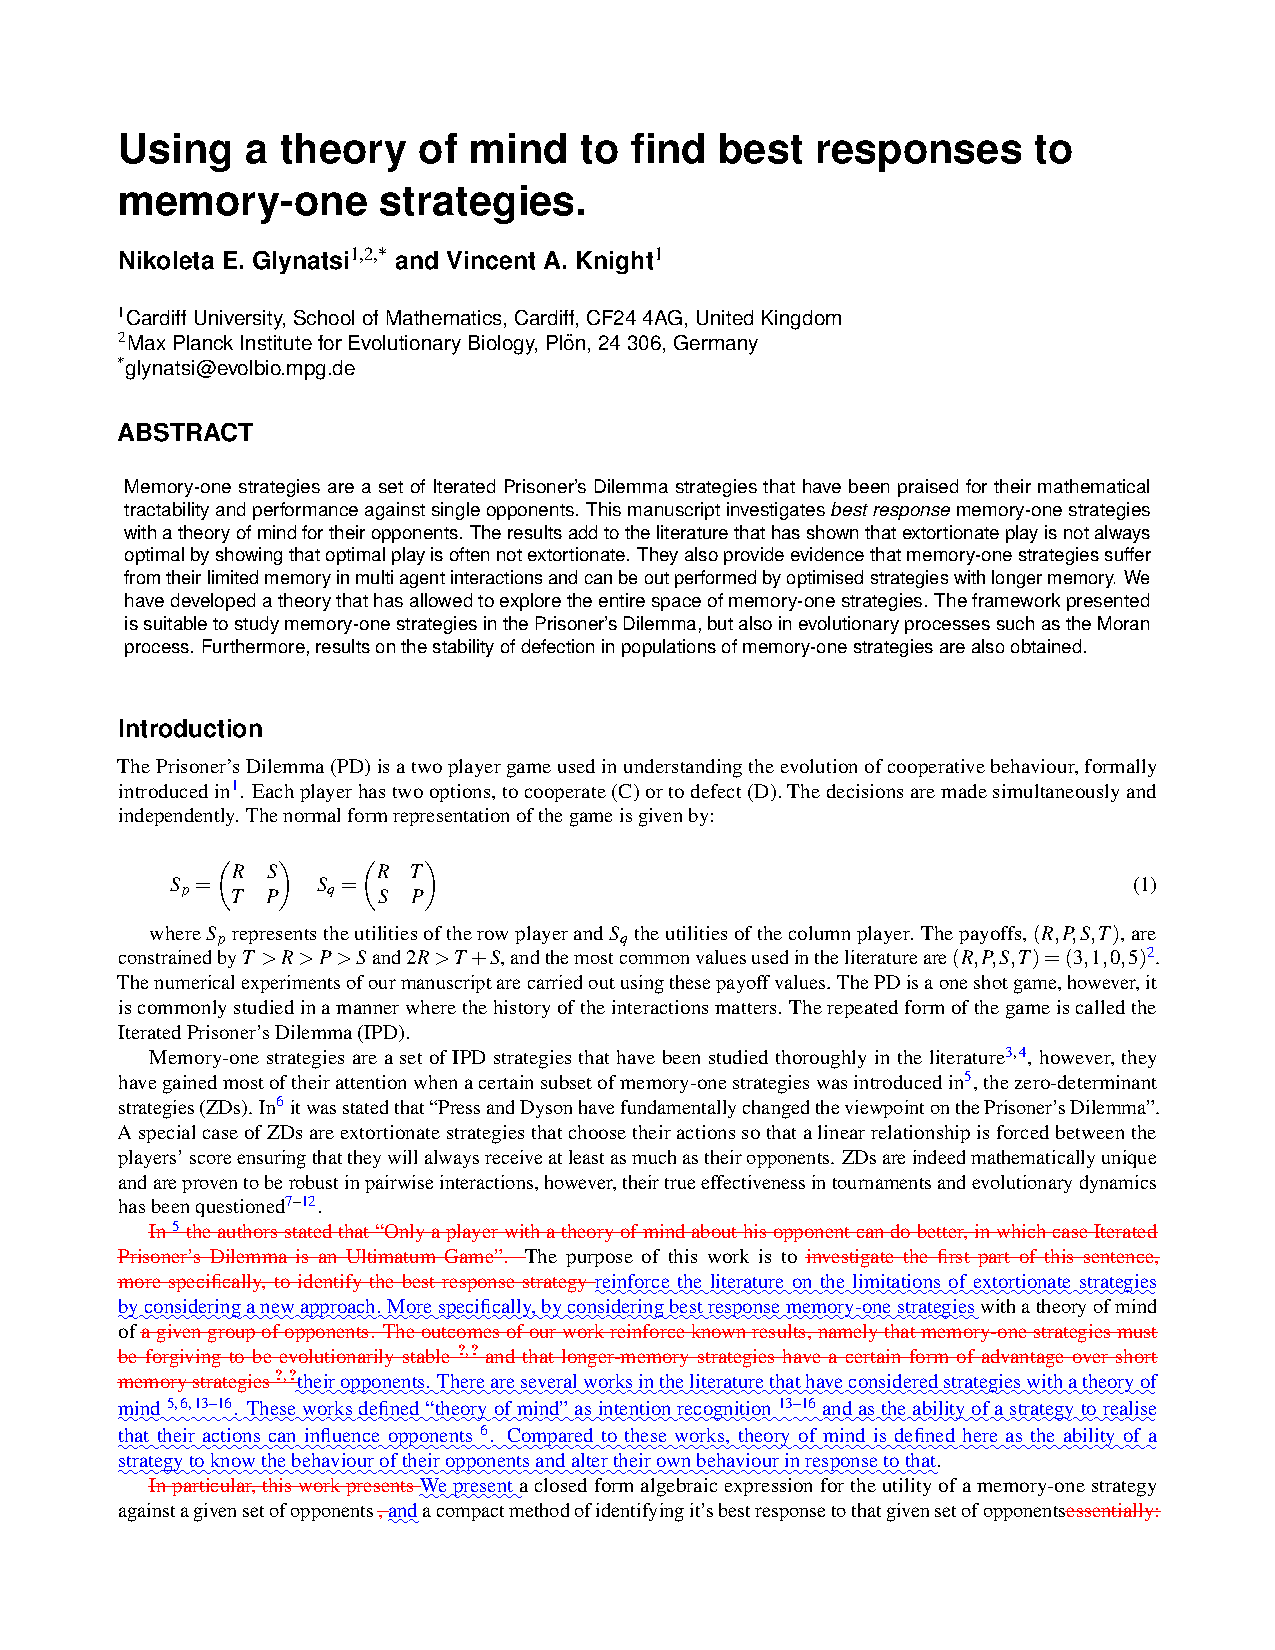
\includepdf[pages=-]{../diff.pdf}

\end{document}
